\documentclass[10pt, oneside]{article} 
\usepackage{amsmath, amsthm, amssymb, calrsfs, wasysym, verbatim, bbm, color, graphics, graphicx, geometry}
\usepackage[most]{tcolorbox}
\usepackage{xcolor}
\usepackage{framed}
\colorlet{shadecolor}{blue!15}
\graphicspath{ {./} }

\geometry{tmargin=.75in, bmargin=.75in, lmargin=.75in, rmargin = .75in}  

\newcommand{\R}{\mathbb{R}}
\newcommand{\C}{\mathbb{C}}
\newcommand{\Z}{\mathbb{Z}}
\newcommand{\N}{\mathbb{N}}
\newcommand{\Q}{\mathbb{Q}}
\newcommand{\Cdot}{\boldsymbol{\cdot}}

\newtheorem{thm}{Theorem}
\newtheorem{defn}{Definition}
\newtheorem{conv}{Convention}
\newtheorem{rem}{Remark}
\newtheorem{lem}{Lemma}
\newtheorem{cor}{Corollary}
\newtheorem{exa}{Example}


\title{Clase \# 2: Propiedades de los fluidos [MF100]}
\author{\textbf{Luis Alejandro Morales}\\ \vspace{0.4cm} Profesor Asistente \\ Universidad Nacional de Colombia-Bogot\'a\\Facultad de Ingenier\'ia \\ Departamento de Ingenieria Civil y Agr\'icola}
\date{Periodo 2022-II}

\begin{document}

\maketitle
\tableofcontents

\vspace{.25in}

\section{Introduccion}
Cualquier caracteristica de un sistema se denomina \textbf{propiedad}. Las propiedades se clasifican en:
\begin{itemize}
\item \textbf{Intensivas}: Aquellas independientes de la masa del sistema como la presion $P$, la temperature $T$ y la densidad $\rho$.
\item \textbf{Extensivas}: Aquellas que dependen del tamano o extension del sistema como la masa total, el volumen total y el momentum total.
\end{itemize}
Un ejemplo para entender la clasificaci\'on de las propiedades es si por ejemplo tenemos un sistema cuyas propiedades son $m$, $V$, $T$, $P$ y $\rho$. Si dividimos en dos partes iguales las propiedades de una de las parter serian $\frac{1}{2}m$, $\frac{1}{2}V$, $T$, $P$ y $\rho$. Note que mientras $T$, $P$ y $\rho$ no cambian al dividir el sistema en dos, $im$ y $V$ son reducidas a la mitad.

Aquellas propiedades extensivas dadas en unidades de masa son llamadas \textbf{propiedades especificas}. El volumne specifico, $v=V/m$, es una propiedad especifica.

Como ya lo sabemos, un fluido esta compuesto por moleculas las cuales pueden estar muy separadas, particularmente los gases. Sin embargo, para el estudio que nos concierne aqui, esa naturaleza atomica de los gases es irrelevante por lo que un fluido es considerado como un medio continuo (sin \"huecos\") y con una homogenea distribucion de la materia, a esto se le denomina el \textbf{continuo}. Esto implica que las propiedades pueden ser analizadas en un punto del espacio y que dichas propiedades varian en el espacio continuamente. 

\section{Propiedades de los campos de velocidad}
\subsection{Descripci\'on Euleriana y Lagrangiana}
Existen dos aproximaciones para analisar problemas en mec\'anica. La primera se centra en el analisis de los campos de flujo y es conocido como el metodo \textbf{euleriano}.  En el metodo euleriano, se calcula la presi\'on del campo de flujo $p(x,y,z,t)$  (e.g en un punto del espacio $x,y,z$ o section) mas no los cambios de presion que experimentar\'ia una part\'icula moviendose en el flujo. Aqui, la posicion del sistema de coordenadas es constante para un intervalo de tiempo (ver Figura~\ref{eulan}).
La segunda aproximaci\'on se centra en seguir particulas individualmente moviendose a traves del flujo, esto es conocido como el metodo \textbf{lagrangiano}. En este, el sistema de coordenadas se mueve con el flujo. El metodo lagrangiano es mas apropiado para el analisis de solidos, mientras que el metodo euleriano esampliamente usado en mecanica de fluidos. 
En mediciones en fluidos, un sensor de presion introducido en un canal de laborario determina la presion del flujo en un punto ($x,y,z$) y en un instante ($t$) determinado. Dicha medicion es acorde con el metodo euleriano. De acuerdo con el metodo lagrangiano,  el mismo sensor arrojado al flujo y moviendose a la misma velocidad permitiria medir la presion de una particula que se mueve con el flujo.

\begin{figure}[h]
\centering
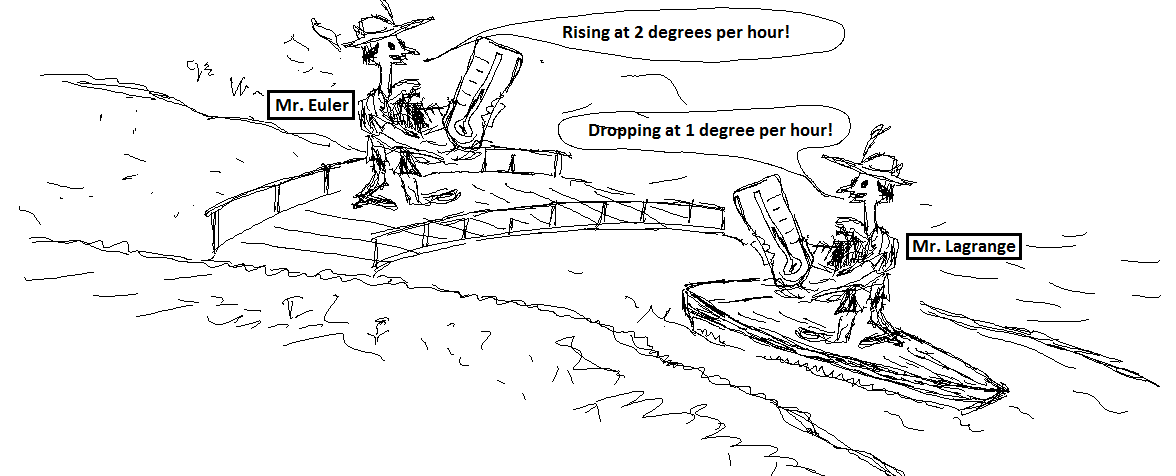
\includegraphics[width=8cm]{MaterialDerivative}
\caption{Sistema euleriano y lagrangiano (http://www.flowillustrator.com/fluid-dynamics/basics/lagrangian-eulerian-viewpoints.php)}
\label{eulan}
\end{figure}

\subsection{El campo de velocidad}
La   propiedad mas conocida de un flujo es el campo de velocidad $\mathbf{V}(x,y,z,t)$, de la cual se derivan otras propiedades. La velocidad es un vector en funcion de la posicion y del tiempo y por lo tanto tiene tres componentes escalares $u$, $v$ y $w$:
$$
\mathbf{V}(x,y,z)=\mathbf{i}u(x,y,z,t) + \mathbf{j}v(x,y,z,t) + \mathbf{k}w(x,y,z,t)
$$

\subsection{El campo de aceleracion}
El vector de aceleracion, $\mathbf{a}=\frac{d\mathbf{V}}{dt}$ es importante en flujos ssometidos a algun tipo de fuerza segun la segunda ley de Newton. El campo de aceleraci\'on de un fluido con respecto a un marco de referencia Euleriano, se define como:
$$
\mathbf{a}=\frac{d\mathbf{V}}{dt}
$$

Si tenemos una  $y=f(u)$ donde $u=g(x)$, $y$ es una funcion compuesta $y=f(g(x))$ y derivable en $x$. De acuerdo con la \textbf{regla de la cadena}, la $\frac{dy}{dx}=\frac{dy}{du} \frac{du}{dx}$. Aplicando dicha regla a la ecuacion anterior tenemos: 

$$
\mathbf{a}=\frac{\partial\mathbf{V}}{dt} + u\frac{\partial\mathbf{V}}{dx} + v\frac{\partial\mathbf{V}}{dy} + w\frac{\partial\mathbf{V}}{dz}
$$

\section{Propiedades termodinamicas de un fluido}
La $\mathbf{V}$ velocidad es la propiedad mas importante de los fluidos, la cual interactua con las propiedades  termodinamicas. Las propiedades mas importantes son:
\begin{itemize}
\item Pressure $p$
\item Density $\rho$
\item Temperature $T$
\end{itemize}

Cuando el balance de calor y energia en un fluido son considerados, las siguientes propiedades son analizadas:
\begin{itemize}
\item Internal energy $\hat{u}$
\item Enthalpy $h=\hat{u}+p/\rho$
\item Entropy $s$
\item Specific heats $c_p$ and $c_v$
\end{itemize}

Por otra parte, los efectos de la fricci\'on y la conducci\'on de calor por dos propiedades del transporte:
\begin{itemize}
\item Coeficiente de viscosidad $\mu$
\item Conductividad t\'ermica $k$
\end{itemize}

Todasd estas nueve propiedades describen el estado del sistema, el cual se entinde como el conjunto de materia que interactual con sus alrededores.

\subsection{Presion}
La presion es el esfuerzo en un punto del espacio en un fluido estatico. Despues, de la velocidad, la presi\'on es la propiedad m\'as din\'amica en la mec\'anica de fluidos. Un gradiente de presion usualmente cause el flujo de un fluido, particularmente en tuberias. La presion en un fluido a baja velocidad puede no ser importante a no ser que esta baje considerablemente causando la formaci\'on de burbujas en el liquido. 

\subsection{Temperatura}
La temperatura $T$ esta relacionada con el nivel de energia interna de un fluido. La temperature  en SI se mide en la \textbf{escala de Kelvin} y la unidades de la temperatura en esta escala es el \textbf{kelvin} ($K$). En el sistema ingles es la \textbf{escala de Rankine} cuyas unidades son el \textbf{rankine} ($R$). Las scalas de la temperature estan relacionadas como sigue:

\begin{equation}
T(K)=T(^oC) + 273.15 = T(R)/1.8
\end{equation}
\begin{equation}
T(R)=T(^oF) + 459.67 = 1.8T(K)
\end{equation}

\subsection{Densidad y gravedad especifica}
La \textbf{densidad} esta definida como la masa ($m$) por unidad de volumen ($V$):
\begin{equation}
\rho = \frac{m}{V} \quad (kg/m^3)
\end{equation}

El reciproco de la densidad es el \textbf{volumen espec\'ifico}, $v$, el cual es definido como el volumen por unidad de masa $v=V/m=1/\rho$.
La densidad de una substance depende de la temperature y de la presi\'on. En la mayoria de los gases $\rho$ es proporcional a la presi\'on e inversamente proporcional a la temperature. En liquidos y solidos, los cuales son considerados incompresibles, la variacion de $\rho$ con respecto a $P$ es despreciable. 
Algunas veces la densidad de un fluido es dada con respecto a una densidad de una sustancia bien conocida. De acuerdo con esto, la \textbf{gravedad espec\'ifica} o \textbf{densidad relativa} se define como la proporci\'on entre la densidad de una sustancia y la densidad de una sustancia conocidad a una temperature especifica (usualmente agua a 4 $^oC$ para la cual $\rho_{H_2 O}=1000 kg/m^3$):

\begin{equation}
SG = \frac{\rho}{\rho_{H_2 O}} 
\end{equation}

La gravedad especifica de algunas substancias es dada en la Tabla~\ref{t1}.

\begin{table}[h!]
\centering
\begin{tabular}{l c}
 \hline
 Substancia & SG \\ [0.5ex]
 \hline\hline
 Agua &  1.0  \\ 
 Sangre (a 37$^oC$) &  1.06  \\ 
 Agua de mar &  1.025 \\ 
 Gasolina &  0.68 \\ 
 Alcohol et\'ilico &  0.790  \\ 
 Mercurio &  13.6  \\ 
 Madera de balsa &  0.17  \\ 
 Madera de roble &  0.93  \\ 
 Oro &  19.3  \\ 
 Hueso &  1.7-2.0  \\ 
 Hielo (a 0$^oC$ &  0.916  \\ 
 Aire & 0.001204  \\ [1ex]
 \hline
\end{tabular}
\caption{Gravedad specifica de algunas substancias a 20$^oC$ y 1$atm$}
\label{t1}
\end{table}


El peso de una unidad de volumen es denominado \textbf{peso espec\'ifico} y si es expresa como:

\begin{equation}
\gamma_s = \rho g \quad (N/m^3)
\end{equation}

donde $g$ es la aceleraci\'on de la gravedad. 

\subsection{Energias potencial y cinematica}
En termoestatica, la energia en una substancia es aquella almacenada en el sistema de acuerdo con la actividad molecular y las fuerzas de atraccion molecular. Esto es denominado comom la \textbf{energia interna} $\hat{u}$ del sistema. Dicha energia interna molecular es funcion de $T$ y $p$ en una substancia. En un fluido en movimiento y de acuerdo con la mecaninca newtoniana, es necesario considerar ademas la energia potencial y la energia cinematica. La energia potencial es igual al trabajo requerido para mover un sistema de masa $m$ desde su origen a una posicion determinada por el vector $\mathbf{r}=\mathbf{i}x + \mathbf{j}y + \mathbf{k}z$ contrarestando el campo gravitacional $\mathbf{g}$. Su valor es $m\mathbf{g}\cdot \mathbf{r}$. La energia cinematica es el trabajo requerido para cambiar la velocidad de un sistema de masa $m$ desde zero a una velocidad $V$. Su valor es $\frac{1}{2}mV^2$. Por lo tanto, la energia total $e$ almacenada en un sistema por unidad de masa en mecanica de fluidos es:
$$
e=\hat{u}+\frac{1}{2}V^2 + (-g\cdot r)
$$
Teniendo en cuenta que $z$ es definido hacia arriba, por lo tanto $\mathbf{g}=-g\mathbf{k}$ y $\mathbf{g}\cdot \mathbf{r}=-gz$, la ecuacion anterior se convierte en:
$$
e=\hat{u}+\frac{1}{2}V^2 + gz
$$

\subsection{Ecuacion de estado de un gas ideal}
Una ecuacion  que relaciona la presi\'on, la temperatura y la densidad (o el volumen espec\'ifico) de una substancia de denomina \textbf{ecuaci\'on de estado}. La ecuaci\'on de estado para substancias en fase gaseosa se conoce como \textbf{ecuaci\'on de estado de un gas ideal} expresada como:

\begin{equation}
Pv=RT  \quad P=\rho R T
\label{idg}
\end{equation}

donde $P$ es la presi\'on absoluta, $v$ es el volumen espec\'ifico, $T$ es la temperatura, $\rho$ es la densidad y $R$ es la constante de los gases. $R$ es diferente para cada gas y se calcula como $R=R_u /M$ donde $R_u$ es la \textbf{constante universal de los gases} igual a 8.314 $kJ/kmol.K$ = 1.986 $Btu/lbmol.R$, y $M$ es la masa molar (peso molecular) de un gas. Valores de $R$ y $M$ para varias substancias estan dados en Tabla A-1. Un gas que obedezca la Ecuaci\'on~\ref{idg} se llama un \textbf{gas ideal}. En un gas ideal el numero de moles es calculado como $N=m/M$ de donde la Ecuaci\'on~\ref{idg} puede escribirse como $PV=mRT$ o $PV=NR_u T$, donde $V$ es el volumen del gas. Para dos gases ideales de masa $m$, el estado de los dos gases se relaciona como $P_1 V_1 / T_1 = P_2 V_2 / T_2$. 

Considerando la relaci\'on entre $P$, $\rho$ y $T$ que describe un gas ideal, si $\downarrow P \quad \uparrow T \Rightarrow \downarrow \rho$ y el gas se comporta como un gas ideal. Gases de baja densidad como el aire, el nitrogeno, el oxigeno, el hidrogeno, el helio, el argon, el neon y el kripton pueden ser analizados como gases ideales. Gases densos como el vapor de agua y aires acondicionados no pueden ser tratados como gases ideales por que estan cerca a un estado de saturaci\'on.

La constante de los gases $R$ tambien puede ser expresada como $R=c_p - c_v$, donde $c_p$ and $c_v$ son los calores especificos. El calor especifico se define como las unidades de calor necesarias para aumentar en $n$ unidades la temperature de un gas de masa $m$. $c_p$ es el calor especifico a una presion constante mientras que $c_v$ es el calor espefifico en un volumen constante. Las unidades de calor especifico en SI son $J.kg^{-1}.K^{-1}$. Para que la Ecuacion~\ref{idg} sea posible, se requiere que la energia molecular interna $\hat{u}$ de un gas perfecto varia solo como funcion de la temperatura: $\hat{u}=\hat{u}(T)$. Por lo tanto el calor especifico $c_v$ varia solo en funcion de la temperatura:
$$
c_v=\left( \frac{\partial \hat{u}}{\partial T}\right)_{\rho} = \frac{d \hat{u}}{dT}=c_v (T) \quad d\hat{u} = c_v (T)dT
$$

De maner similar, $h$ y $c_p$ de un gas perfecto varia en funci\'on de la temperatura:
$$
h=\hat{u} + \frac{p}{\rho}=\hat{u}+RT=h(T)
$$
$$
c_p=\left( \frac{\partial h}{\partial T}\right)_{p} = \frac{d h}{dT}=c_p (T) \quad dh = c_p (T)dT
$$

El radio de los calores especificos de un gas perfecto es un parametro adimencional importante en el analisis de flujo compresible:
$$
k = \frac{c_p}{c_v}=k(T) \geq 1
$$
Como una primera aproximacion en problemas de flujo de aire, $c_p$, $c_v$ y $k$ son tomadas como como constantes:
$$
k\approx 1.4
$$
$$
c_v = \frac{R}{k-1} \approx 4293\ ft^2/(s^2 . ^oR) = 718\ m^2/(s^2 . K)
$$
$$
c_p = \frac{kR}{k-1} \approx 6010\ ft^2/(s^2 . ^oR) = 1005\ m^2/(s^2 . K)
$$
Para todos los gases, $c_p$ y $c_v$ increase gradualmente con la temperature mientras $k$ decrece gradualmente. 

\subsection{Relacion de estado para los luquidos}
Liquidos son considerados incompresibles por lo que su calor espefico es constante. Por lo tanto una relacion de estado ideal para un liquido es:
$$
\rho \approx const \quad c_p \approx c_v \approx const  \quad dh\approx c_p dT
$$
En un liquido, la densidad decrese un poco con la temperature e incrementa moderadamente con la presion. Si despreciamos los efectos de la temperature, se puede establecer la siguiente relacion empirica entre la presion y la densidad:
$$
\frac{p}{p_a}\approx (B+1) \left( \frac{\rho}{\rho_a} \right)^n - B
$$
donde $B$ y $n$ son parametros adimensionales que varian levemente con la temperatura, y $p_a$ y $\rho_a$ son valores estandard de la presion y la densidad atmosferica. Para el agua, $B\approx3000$ y $n=7$.

En el caso del agua de mar, por ser una mezcla de sal y agua, se requieren tres propiedades termodinamicas para definir su estado: presion, temperatura y salinidad $\hat{S}$, esta ultima calculada como el peso de la sal disuelta divida por el peso de la mezcla. La salinidad promedio del agua de mar es 0.035 o usualmente escrita como 35 partes por 1000. La densidad promedio de agua de mar es 2.00 $slugs/ft^3$ $\approx$ 1030 $kg/m^3$. El agua de mar tiene tres calores especificos, todos approximadamente iguales al del agua pura 25200 $ft^2/(s^2. ^oR)$ = 4210 $m^2/(s^2. K)$.

\section{Viscosidad}
La \textbf{viscosidad} es una medida de la resistencia de un fluido a fluir. Esta determina la tasa de deformaci\'on de un fluido que es generada cuando este es sometido a un esfuerzo cortante $\tau$. Por ejemplo es mucho mas facil moverse en aire que en el agua, ya que esta ultima tiene una viscosidad 50 veces mas alta (ver Figura~\ref{visco0}). Mucho mas dificil es el movimiento en aceite que podria tener 300 veces mas viscosidad que el agua. 

% Fig 2.23 Cengel 
\begin{figure}[h]
\centering
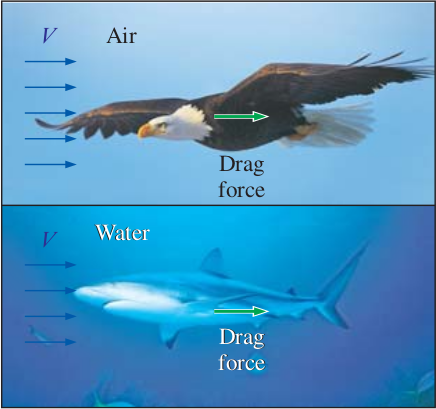
\includegraphics[width=8cm]{visco0}
\caption{El fluido ejerce una fuerza de atrastre sobre el cuerpo en movimiento debido a la friccion causada por la viscosidad.}
\label{visco0}
\end{figure}



Si consideramos un fluido que se mueve a una velocidad $u$ en un plano horizontal como resultado de una fuerza horizontal la cual produce un esfuerzo cortante, tenemos que el angulo de deformaci\'on $\delta \theta$ crece continuamente con el tiempo si $\tau$ se mantine (ver Figura~\ref{visco}).

% Fig 1.6 White
\begin{figure}[h]
\centering
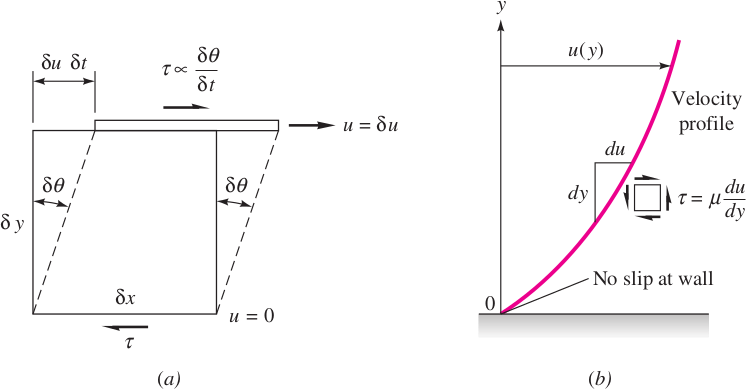
\includegraphics[width=8cm]{visco}
\caption{a)Deformacion de un fluido que flujo sobre una superficie horizontal a velocidad $u$ y  b) perfil de velocidades de fluido en la capa l\'imite.}
\label{visco}
\end{figure}

Por lo tanto, en fluidos como el agua, el aceite o el aire, la tasa de deformacion se relaciona linealmente con el esfuerzo:
\begin{equation}
\tau \propto \frac{\delta \theta}{\delta t}
\label{vis1}
\end{equation}

De la figura~\ref{visco}a:
$$
\tan \delta \theta = \frac{\delta u \delta t}{\delta y}
$$
En el limite infinitesimal cuando $\delta \theta$ se hace pequen\~no, $\tan \delta \theta \approx \delta \theta$ y la ecuacion anterior se comvierte en:
$$
\frac{d\theta}{dt}=\frac{du}{dy}
$$
la cual expresa la equivalencia entre la tasa de deformacion y el gradiente de velocidad. Reemplazando en la ecuaci\'on~\ref{vis1} y teniendo en cuenta que la constante de proporcionalidad es el coeficiente de viscosidad $\mu$:

\begin{equation}
\tau = \mu \frac{d \theta}{d t} = \frac{d u}{d y}
\label{vis2}
\end{equation}

$\mu$ tiene dimensiones ${FT/L^2}$ o ${M/(LT}$, en SI son $kg/m.s$ y en BG son $slugs/ft.s$. Los fluidos que se comportan de acuerdo con la ecuacion~\ref{vis2} son denominados \textbf{fluidos newtonianos}.

Si analisamos el perfil de velocidades en la \textbf{capa limite} (ver Figura\ref{visco}b) la cual es la capa de fluido mas cercana a la placa solida inferior, la velocidad $u \approx 0$ y $\tau$ es m\'aximo en cercanias a la placa solida. Dicho fenomeno es conocido como la \textbf{condicion de no deslizamiento} en fluidos viscosos. 

La viscocidad es una propiedad termodinamica de los fluidos que depende de la presion $p$ y de la temperatura $T$. Sin embargo, la variacion de $\mu$ con respecto a la presion es menor, mientras qwue la variacion con respecto a la temperatura es significativa.


Un problema  clasico es el flujo inducido entre una placa inferior fija y una placa superior que se mueve a una velocidad $\mathbf{V}$ (ver Figura~\ref{pla}). La distancia entre las placas es $h$ y dicho espacio esta ocupado por un fluido newtoniano. Si las placas son grandes, el movimiento permanente induce una distribucion de velocidad $u(y)$  (ver Figura~\ref{pla}) en donde $v=w=0$ y la aceleracion es zero. De acuerdo con lo anterior, a un balance de fuerza sobre un elemento de fluido resulta en un esfuerzo constante en cualquier punto del fluido. Por tanto la Equacion~\ref{vis2} se convierte en:

% Fig 1.8 White
\begin{figure}[h]
\centering
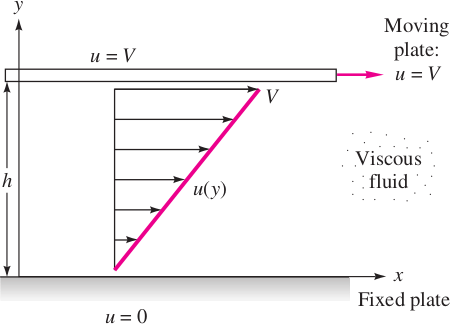
\includegraphics[width=8cm]{plate}
\caption{Flujo viscoso inducido por el movimiento relativo de dos placas paralelas.}
\label{pla}
\end{figure}

$$
\frac{du}{dy}=\frac{\tau}{\mu}=\text{const}
$$
Integrando esta ecuacion para $u$, tenemos
$$
u=a+by
$$
lo cual indica una distribucion lineal de la velocidad tal como se muestra en la Figura~\ref{pla} en donde $a$ y $b$ son constantes que se evaluan como:
$$
u= 
\begin{cases}
0 = a+b(0) & \quad \text{en}\ y=0 \\
V = a+b(h) & \quad \text{en}\ y=h 
\end{cases}
$$
de donde $a=0$ y $b=V/h$. Reemplazando en la ecuacion, el perfil de velocidades entre las placas esta dato por:
\begin{equation}
u=V\frac{y}{h}
\label{upl}
\end{equation}


\subsection{El Numero de Reynolds}
El numero de Reynolds $Re$ es un numero adimensional que caracteriza el movimiento de un fluido y se define como:
\begin{equation}
Re=\frac{\rho VL}{\mu}=\frac{VL}{\nu}
\label{re1}
\end{equation}
donde $V$ es la velocidad, $L$ es la longitud caracteristica del flujo y $\nu=\mu/\rho$  es la \textbf{viscosidad cinematica}. La ecuacion~\ref{re1} indica que $Re$ es la relacion de las fuerzas convectivas o inerciales y las fuerzas viscosas presentes en el fluido. De acuerdo con esto, $Re$ muy bajos significan flujos muy viscosos donde las fuerzas inerciales son despreciables. $Re$ moderados son flujos \textbf{laminares} que se mueven suavemente en capas paralelas. Un $Re$ alto es caracteristico de un flujo \textbf{turbulento}.  

\subsection{Variacion de la viscosidad con la temperatura}
La viscosidad de un gas incrementa con la temperature. De acuerdo con esto existen dos leyes al respecto:
\begin{equation}
\frac{\mu}{\mu_0} \approx 
\begin{cases}
\left( \frac{T}{T_0} \right)^n & \quad \text{ley de potencia} \\
\frac{(T/T_0 )^{3/2}(T_0 + S)}{T+S} & \quad \text{ley de Sutherland} 
\end{cases}
\label{vist}
\end{equation}

donde $\mu_0$ es la viscosidad a una temperature absoluta $T_0$ (usualmente 273 K). Las constantes $n$ y $S$ son constantes ajustadas con base en datos. Por ejemplo para aire, $n\approx 0.7$ y $S\approx 110$ 

En liquidos, la viscosidad decrece con la temperatura de una forma casi exponencial $\mu \approx ae^{-bT}$. Con base en esta ecuacion esta expresion es derivada:
\begin{equation}
\ln \frac{\mu}{\mu_0} \approx  a + b \left(\frac{T_0}{T}\right)+ c\left(\frac{T_0}{T}\right)^2
\label{visf}
\end{equation}

en donde para agua con $T_0 = 273.16\ K$ y $\mu = 0.001792\ kg/(m.s)$, $a=-1.94$, $b=-4.80$ y $c=6.74$ con una  exactitud del $\pm 1$ \%.

\subsection{Fluidos no newtonianos}
Fluidos que no siguen la equacion lineal ~\ref{vis2} son llamados \textbf{no newtonianos}. Mientras que en los flujos newtonianos la viscosidad es constante con el aumento del esfuerzo, en los fluidosno newtonianos la viscosidad cambia. Algunos tipos de fluidos no newtonianos son:

% Fig 2.26 Cengel
\begin{figure}[h]
\centering
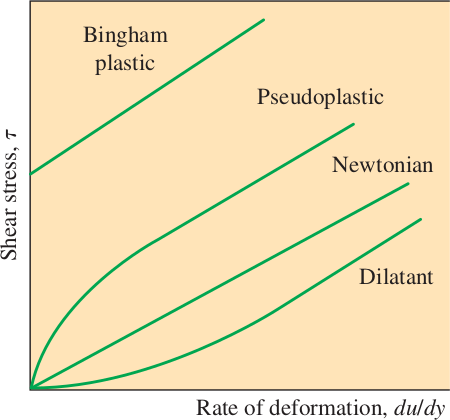
\includegraphics[width=8cm]{nonew}
\caption{Variacion del esfuerzo con la tasa de deformacion para fluidos newtonianos y no newtonianos.}
\label{nonew}
\end{figure}

\begin{itemize}
\item \textbf{Dilatante}: Increase its resistencia cuando la tasa de deformacion incrementa.
\item \textbf{Seudoplastico}: La resistencia disminuye a altas tasas de deformacion. Por ejemplo: pintura y soluciones de polimeros. La pintura es gruesa antes de aplicarla pero se hace delgada cuando se aplica a una alta taza de deformacion.
\item \textbf{Bingham plastico}: Requieren un esfuerzo inicial antes de que inicie a fluir o deformarse. Por ejemplo: mayonesa, crema de dientes, lodos, salsa de tomate. La salsa de tomate no sale del recipiente a menos que se le aplique un esfuerzo inicial (se sacuda o se exprima el recipiente). 
\end{itemize}

\subsection{Tensi\'on superficial}

\begin{figure}[h]
\centering
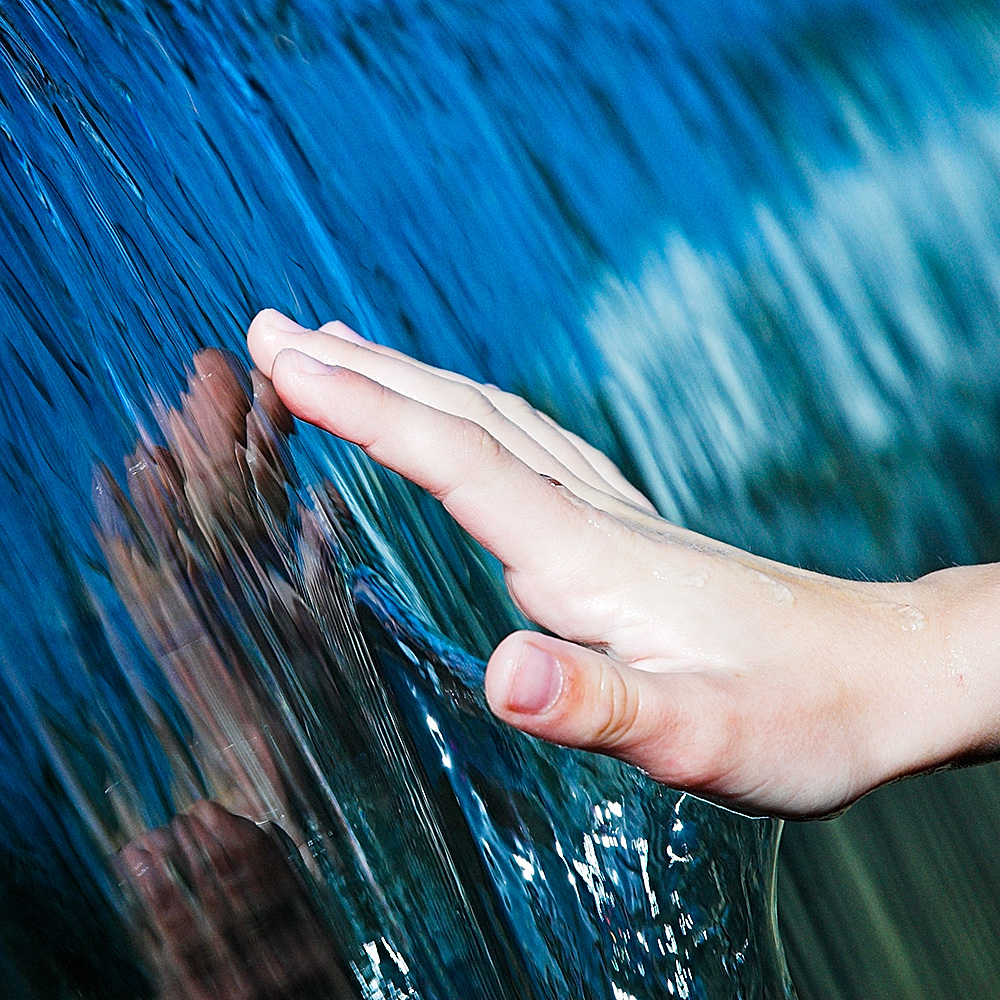
\includegraphics[width=8cm]{SurfaceTension}
\end{figure}


En una superficie de contacto entre dos fluidos diferentes (e.g aire y agua) se forma una interface en donde fuerzas de tension actuan para mantener la cohesion del fluido. La magnitud de esta fuerza por unidad de longitud es llamada \textbf{tensi\'on superficial}. Si cortamos una seccion $dl$ de la superficie de interface, fuerzas iguales y opuestas cuya magnitud es $\Upsilon\ dl$ actuan normal al corte y paralelas a la superficie. $\Upsilon$ es conocido como el \textbf{coeficiente de tensi\'on superficial} y sus dimensiones  son ${F/L}$; $N/m$ en SI y $lbf/ft$ en BG.

Dos interfaces comunes son: agua-aire y mercurio-aire. Para una superficie limpia a 20$^oC$, $\Upsilon$ es estimado igual a:
\begin{equation}
\Upsilon =
\begin{cases}
0.0050\ lbf/ft = 0.073\ N/m & \quad \text{air-water} \\
0.033\ lbf/ft = 0.48\ N/m& \quad \text{air-mercury} 
\end{cases}
\end{equation}

Estos values pueden variar considerablemente si por ejemplo la superficie contienen contaminantes como detergentes o si la temperature del fluido cambia (e.g. $\Upsilon\ \downarrow$ cuando $T\ \uparrow$).

Si la interface es curva, el balance mecanico muestra que existe diferencias de presion en diferentes puntos sobre la superficie, en donde las presiones mayores existen sobre la parte concava de la interface (ver figura~\ref{tesu}. En la figura~\ref{tesu}a, el incremento de presion al interior de la superficia es balanceada por las fuerzas de tensi\'on:

% Fig 1.11 White
\begin{figure}[h]
\centering
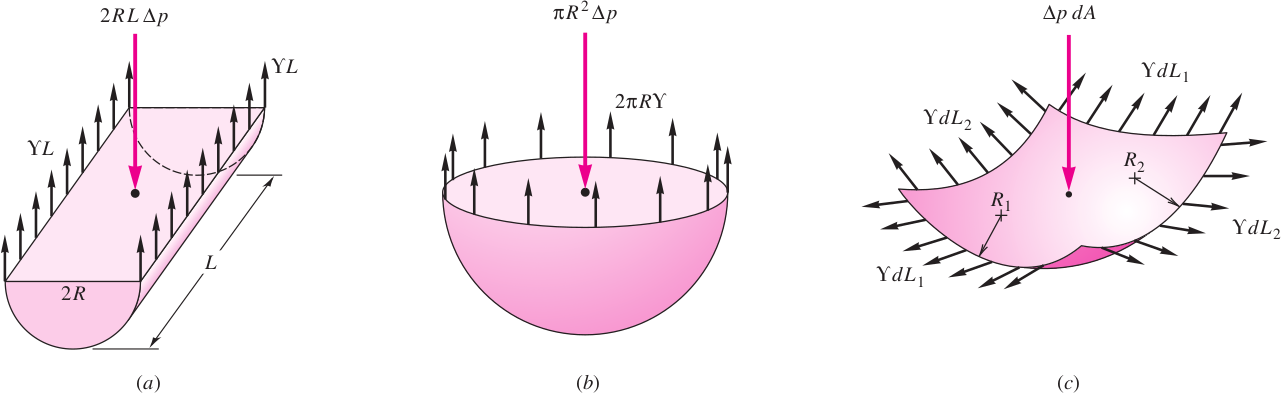
\includegraphics[width=10cm]{tesu}
\caption{Cambios de presi\'on sobre la interface curva debido a la tension superficial a) en el interior de un liquido con forma cilindrica, b) al interior de una gota esferica de liquido y c) al interior de una interface curva general.}
\label{tesu}
\end{figure}

\begin{equation}
2RL \Delta p = 2 \Upsilon L \quad \Delta p = \frac{\Upsilon}{R}
\end{equation}

en donde el peso del liquido no es considerado. Al interior de una gota esferica de liquido (figura~\ref{tesu}b), el balance de fuerzas es:

\begin{equation}
\pi R^2 \Delta p = 2 \pi R \Upsilon \quad \Delta p = \frac{2\Upsilon}{R}
\end{equation}

En el caso de una burbuja de jabon, la cual tiene una interface interna y externa con el aire, cuyos radios son aproximadamente iguales $R$, el balance de fuerzas es:
\begin{equation}
\Delta p_{burbuja} \approx 2 \Delta p_{gota} = \frac{4\Upsilon}{R}
\end{equation}

Para el caso general de una interface curva arbitraria, cuyos radios de curvatura principales son $R_1$ y $R_2$, el balance de fuerzas normal a la superficie  muestra que el incremento de presion en la parte concava es:
\begin{equation}
\Delta p = \Upsilon (R^{-1}_1 + R^{-1}_2)
\label{ts1}
\end{equation}

Notara que las ecuaciones anteriores podrian haber sido derivadas a partir de la ecuacion~\ref{ts1} si $R_1 = R$ y $R_2 = \inf$.


\subsubsection{Efecto capilar}
Otra consecuencia interesante de la tension superficial es el \textbf{efecto capilar} el cual es el incremento o la reduccion de un liquido en un tubo de diametro pequeno al insertarse en dicho liquido (ver figura~\ref{efc}). La superficie libre del liquido en el tubo se llama \textbf{menisco}. 

% Fig 2.36 Cengel
\begin{figure}[h]
\centering
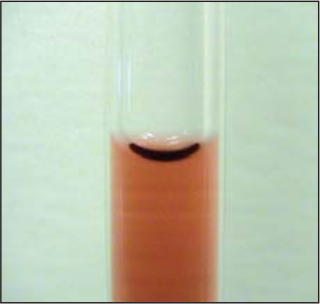
\includegraphics[width=10cm]{ecapilar}
\caption{Efecto capilar en un tubo de 4mm de diametro con agua de color.}
\label{efc}
\end{figure}


Gracias al efecto capilar, en un vaso con agua se puede observar que la superficie del agua se curva cerca a las paredes del vaso formando un \textbf{angulo de contacto} $\phi$. Algo opuesto occurre con el mercurio (ver figura~\ref{eca}). De acuerdo con esto, un liquido moja las paredes del vaso si $\phi < 90^o$, para el caso en que no mojaria las paredes $\phi > 90^o$. 

% Fig 2.35 Cengel
\begin{figure}[h]
\centering
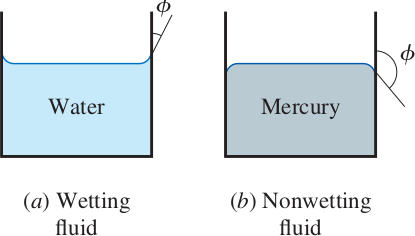
\includegraphics[width=10cm]{ecangulo}
\caption{Angulo de contacto en el a) agua y en el b) mercurio.}
\label{eca}
\end{figure}

El efecto capilar occurre debido a que las fuerzas de tension superficial en la interface de contacto (fuerzas adesivas) tienden a elevar el fluido en cercanias a esta interface. El equilibrio se presenta cuando el peso iguala dicha tensi\'on superficial (fuerzas cohesivas). En el mercurio, las fuerzas cohesivas son mucho mayores que las fuerzas adesivas en la interface lo cual crea distaciamento de las paredes.  

La magnitud de la elevacion capilar $h$  en un tubo circular se puede determinar a partir de un balance de fuerzas (ver figura~\ref{ecfu}). Note que la fuerzas por presion atmosferica son iguales dentro y por fuerza del tubo, dicha fuerzas se anulan.  

% Fig 2.38 Cengel
\begin{figure}[h]
\centering
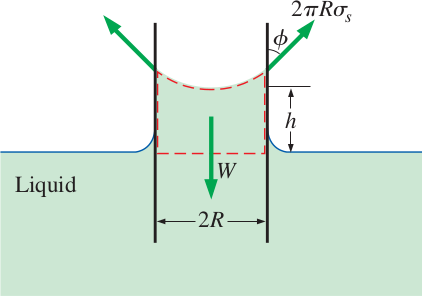
\includegraphics[width=10cm]{ecfuer}
\caption{Fuerzas que actuan sobre una column de liquido en un tubo debido al efecto capilar.}
\label{ecfu}
\end{figure}

El peso de la columna de liquido es:
$$
W = mg = \rho V g = \rho g (\pi R^2 h)
$$

Igualando el peso a la componente vertical de la tension superficial:
$$
W=F_{surface} \rightarrow \rho g (\pi R^2 h) = 2\pi R \Upsilon \cos \phi
$$

Por lo tanto, la elevacion capillar es:
\begin{equation}
h=\frac{2 \Upsilon}{\rho g R} \cos \phi
\label{crise}
\end{equation}

 Si tenemos mercurio, por ejemplo, tenemos una caida capillar, que es igual a -$h$ ya que  $\phi > 90^o$ $\cos \phi$ es negativo. Notara que en la ecuaci\'on~\ref{crise}, cuando $R$ o $\rho$ disminuyen $h$ aumenta.  

\section{Presi\'on de vapor}
La \textbf{presion de vapor} es la presion a la cual un liquido hierve y esta en equilibrio con su propio vapor. Por ejemplo, la presion de vapor del agua a 68 $^o$F es 49 $lbf/ft^2$ mientras que la del mercurio es solo 0.0035 $lbf/ft^2$. Si la presion en el liquido es mayor que la presion de vapor, el intercambio entre el liquido y el vapor es por evaporacion en la interface. Si la presion del liquido cae por debajo de la presion de vapor, burbujas empiezan a aparecer en el liquido. Si el agua es calentada a 212 $^o$F, su presion de vapor aumenta a 2116 $lbf/ft^2$ y el agua a presion atmosferica empieza a hervir. Cuando la presion de liquido cae por debajo de la presion de vapor debido a un fenomeno de flujo, esto es conocido \textbf{cavitaci\'on}. El numero de cavitacion es:

% Fig 2.38 Cengel
\begin{figure}[h]
\centering
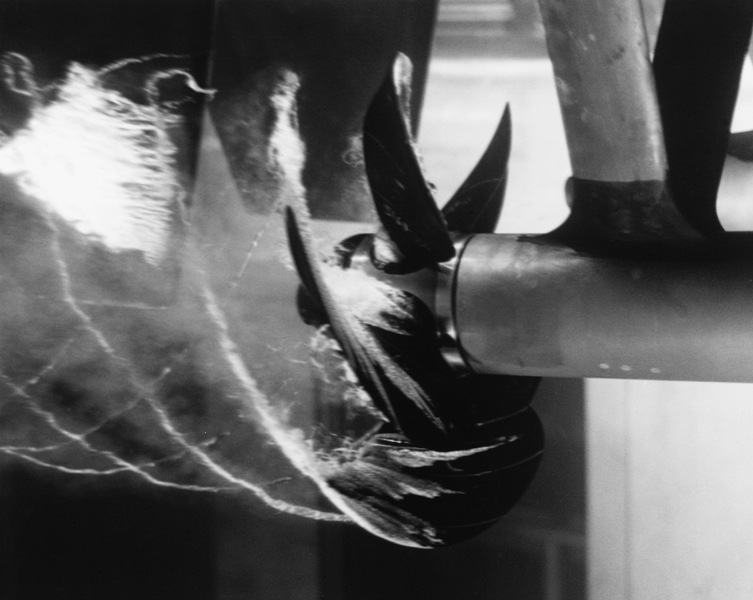
\includegraphics[width=10cm]{Cavitating-prop}
\caption{Cavitacion en una helice en un canal de agua.}
\label{cavi}
\end{figure}

\begin{equation}
Ca = \frac{p_a - p_v}{\frac{1}{2}\rho V^2}
\label{can}
\end{equation}
donde $p_a$ es la presion ambiental, $p_v$ es la presion de vapor, $V$ es la velocidad del flujo y $\rho$ es la densidad del fluido.


\section{Velocidad del sonido}
Un parametro importante en el estudio de flujo compresible es la \textbf{velocidad del sonido}, definida como la velocidad a la cual una pequena onda de presion, creada por una perturbacion local, viaja a traves de un medio (e.g. fluido). En temas futuros, veremos que con base en la termodinamica y el momentum, la velocidad del sonido $a$ es definida como la derivada de la presion con respecto a la densidad y es proporcional al modulo isentropico $B$ (el cual mide la compresibilidad del fluido bajo cambios de presion:
\begin{equation}
a^2 = \frac{B}{\rho} = \left (\frac{\partial p}{\partial \rho} \right )_s = k \left (\frac{\partial p}{\partial \rho} \right )_T 
\label{vso}
\end{equation}

donde $k=\frac{c_p}{c_v}$ es el radio de calor especifico y los subindices $s$ y $T$ indican a entropia y temperatura constante, respectivamente. Note que $B= \rho \left (\frac{\partial p}{\partial \rho} \right )_s$. 

Cuando el fluido es  un gas ideal ($P=\rho RT$), usando la equacion~\ref{vso}, la velocidad del sonido es:
\begin{equation}
a^2 = k \left (\frac{\partial p}{\partial \rho} \right )_T = k \left[ \frac{\partial (\rho RT)}{\partial \rho} \right]_T = kRT
\end{equation}
o
\begin{equation}
a = \sqrt{kRT}
\end{equation}

donde $R$ es la constante de los gases $T$ es la temperatura absoluta. 

Otro importante parametro en fluidos compresibles es el \textbf{numero de Match} definido como:
\begin{equation}
Ma = \frac{V}{a}
\end{equation}
donde $V$ es la velocidad del fluido. Note que como $Ma$ depende de $a$ la cual depende del estado del fluido, para un avion que viaja a una velocidad constante $Ma$ puede ser diferente a diferentes localizaciones.


\end{document}
